\documentclass[a4paper]{article}

\usepackage[utf8]{inputenc}
\usepackage[T1]{fontenc}
\usepackage[english]{babel}
\usepackage{color}
\usepackage{listings}
\usepackage{graphicx}


\usepackage{amsmath}
\usepackage{amsthm}
\usepackage{amssymb}

\usepackage{algorithmicx}
\usepackage{algpseudocode}


\definecolor{darkgray}{rgb}{0.4, 0.4, 0.4}
\definecolor{purple}{rgb}{0.65, 0.12, 0.82}

\lstdefinelanguage{xUnicorn}%
  {morekeywords={graph,cluster,node,boolean,config,or,and,port,attr},%
   sensitive=true,%
   morecomment=[s]{/*}{*/},%
   morecomment=[l]{//},
   morestring=[b]",%
  }%
\lstset{
    language={xUnicorn},
    tabsize=2,
    basicstyle=\footnotesize\ttfamily,
    numbers=left,
    numberstyle=\tiny,
    xleftmargin=2em,
    framexleftmargin=1.5em,
    flexiblecolumns=false,
    frame=none,
    captionpos=b,
    aboveskip=0pt,belowskip=0pt,showstringspaces=false,
    % Code design
    identifierstyle=\color{black},
    keywordstyle=\color{blue}\bfseries,
    stringstyle=\color{purple}\ttfamily,
    commentstyle=\color{darkgray}\ttfamily,
    escapeinside={@}{@}
}


\graphicspath{{./images/}}

\title{Unicorn}
\date{}
\author{}

\begin{document}
\maketitle

\section*{Example}
\begin{lstlisting}
@\label{prgex:graph}@graph prg {
@\label{prgex:node}@    node Entry {
        port out[L2EtherClassified] }

@\label{prgex:cluster}@    cluster L2Ether {
@\label{prgex:boolnode}@        boolean Classified {
            port true[ValidType]
            port false[] }

        boolean ValidType {
            port true[CValidCRC]
            port false[] }

@\label{prgex:confignode}@        config CValidCRC {
            port true[ValidCRC]
            port false[ValidBroadcast ValidBroadcast_
                       ValidUnicast ValidUnicast_] }

        boolean ValidCRC {
            port true[ValidBroadcast ValidBroadcast_
                      ValidUnicast ValidUnicast_]
            port false[] }

        boolean ValidUnicast_ {
            port true false[ValidDest] }

        boolean ValidBroadcast_ {
            port true false[ValidDest] }

        // Software nodes for the unicast/broadcast tests
        boolean ValidUnicast {
@\label{prgex:attr}@            attr "software"
            port true false[] }
        boolean ValidBroadcast {
            attr "software"
            port true false[] }

@\label{prgex:ornode}@        or ValidDest {
@\label{prgex:cref}@            port true[.Queue0]
            port false[] }
    }

@\label{prgex:gconfig}@    config QueueN {
@\label{prgex:gconfigfun}@        function queueConfig
        port out[] }
}
\end{lstlisting}

\begin{figure}[h]
\noindent\makebox[\textwidth]{
  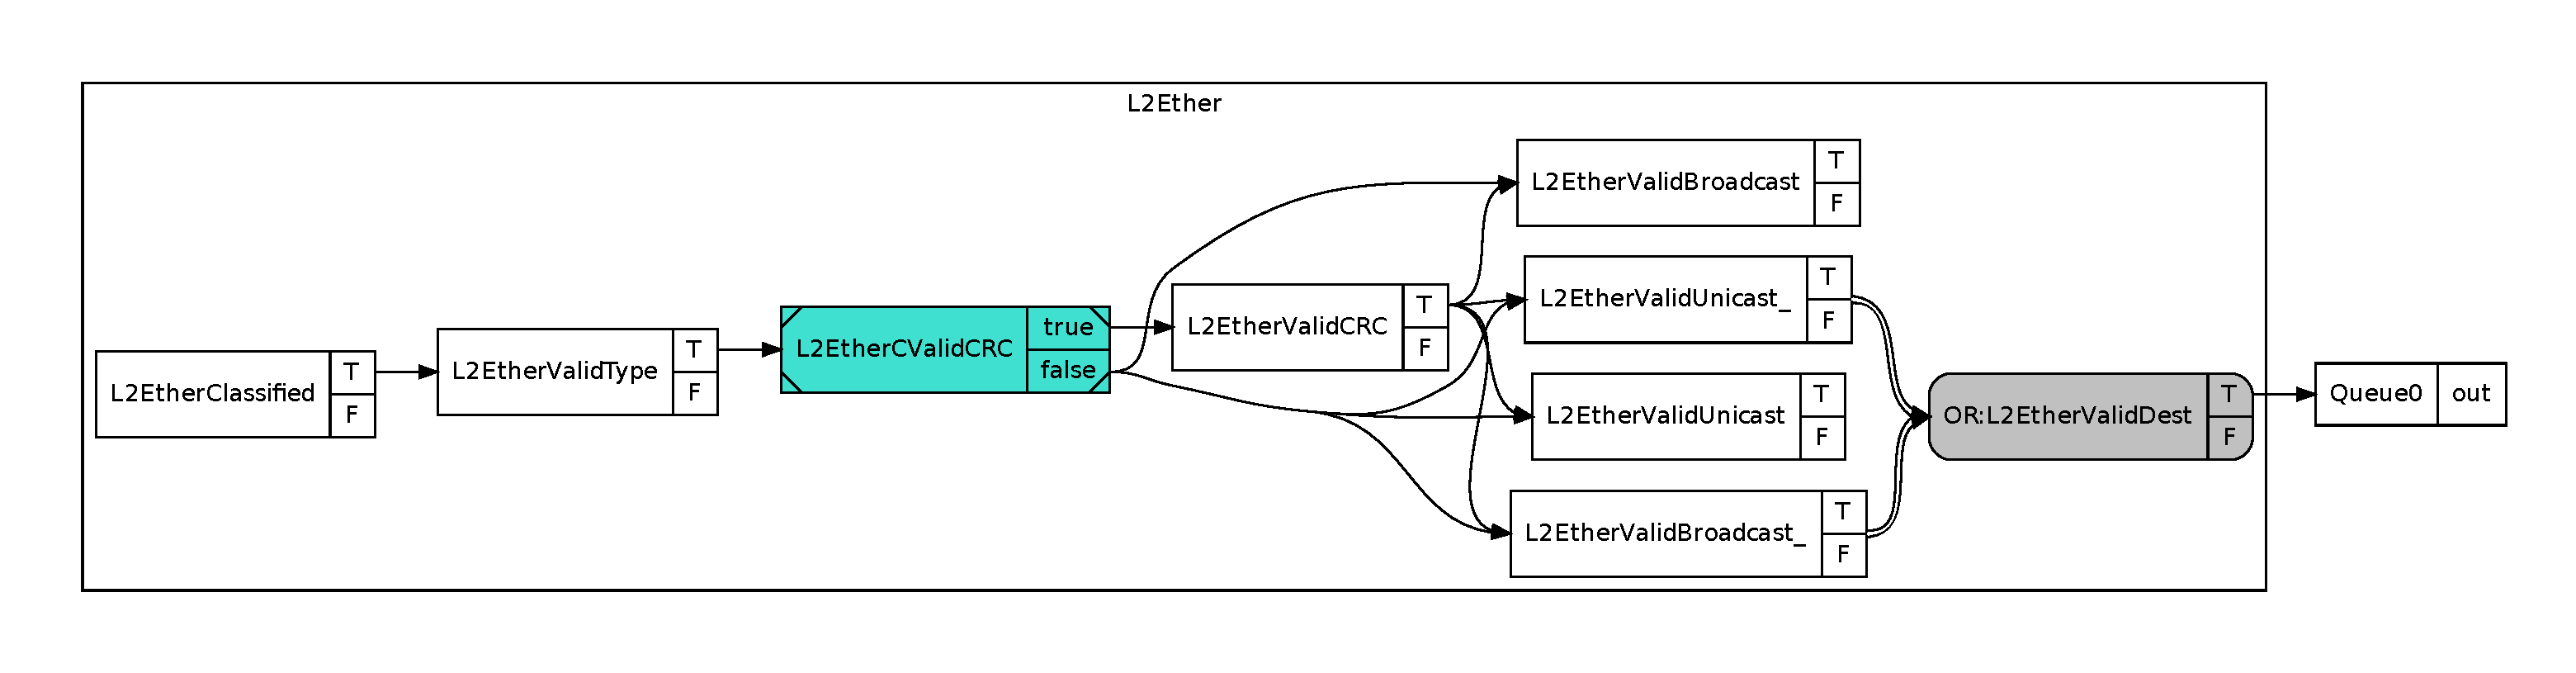
\includegraphics[width=1.7\textwidth]{prg_example}
}
\caption{Graph corresponding to the Unicorn example above}
\label{fig:exfig}
\end{figure}

The example above shows a simple PRG defined in Unicorn for basic Ethernet
functionality, the graph is shown in figure~\ref{fig:exfig}. Multiple different
node definitions are shown, starting with \texttt{boolean}, \texttt{config},
\texttt{or} and \texttt{node}. The most general class of nodes is defined by
\texttt{node} as shown on line~\ref{prgex:node}, and can have arbitrary ports.
Boolean nodes such as shown on line~\ref{prgex:boolnode} are required to have
exactly two ports: \texttt{true} and \texttt{false}. While both general and
boolean nodes carry node-specific implementations, the boolean operation nodes
\texttt{and}/\texttt{or} such as defined on line~\ref{prgex:ornode} all
implement the same logical functions. For all node types attributes can be
specified using \texttt{attr} as shown on line~\ref{prgex:attr}.


\texttt{config} nodes (lines \ref{prgex:confignode} and \ref{prgex:gconfig})
represent configuration node, that will be transformed into a specific subgraph
depending on the configuration to be applied. There are two different types of
configuration nodes, simplified configuration nodes as show on
line~\ref{prgex:confignode} and general configuration node as on
line~\ref{prgex:gconfig}. For simplified configuration nodes applying a specific
configuration will result in the node being removed and the incoming edges
replaced by edges leading directly to the nodes referred to by the chosen port
of the configuration node. General configuration nodes are implemented by
specifying a Haskell function name (line~\ref{prgex:gconfigfun}) that will
generate the subgraph. The following listing shows an example for such a
configuration function:

\begin{lstlisting}[language=haskell]
queueConfig ::
    [(Node,String)] ->
    [(String,Node)] ->
    String ->
    [(Node,String,Node)]
queueConfig inE outE cfg = map (\(a,b) -> (a,b,queueN)) inE
    where queueN = getDecNode ("Queue" ++ cfg) "" (NaryNode []) []
\end{lstlisting}

The first parameter describes the incoming edges to the configuration nodes, the
second parameter is a list of outgoing edges, and the third parameter specifies
the configuration value. As a result the function has to return a subgraph
specified as a set of edges. Note that subgraph should be self-contained,
meaning that there must be no edges leading to other nodes of the graph besides
the incoming and outgoing edges passed as parameters.


Nodes can be grouped into clusters as shown on line~\ref{prgex:cluster}. Node
names in a cluster will be prefixed with the cluster name, this applies both to
node names for node definition as well as node references for ports. This
behaviour can be overridden by prefixing the node name by a dot as shown on
line~\ref{prgex:cref}. Clusters can also be nested in which case each dot at the
beginning of an identifier strips one cluster starting with the innermost cluster.




\section*{Implementation}
The implementation of the Unicorn DSL is based on Haskell QuasiQuotes.
QuasiQuotes allow implementations of embedded DSLs in Haskell that are
translated to Haskell code at compile time. The following listing shows a
Haskell example:

\begin{lstlisting}[language=haskell]
{-# LANGUAGE QuasiQuotes #-}

import Unicorn
import qualified Operations as OP
import DotGenerator as DG

[unicorn|
graph prg {
  ...
}
|]

main = do
    putStrLn (DG.toDotClustered prgClusters prgNodes)
\end{lstlisting}

The generated code includes a Haskell function for each node that returns a
Haskell representation of the node. The name of the function is composed of the
graph name (as specified on line~\ref{prgex:graph} of the PRG example above) and
the node name, such as for example \texttt{prgL2EtherClassified} for the first
node. In addition an association list of clusters to nodes will be defined, in
the case of the example above named \texttt{prgNodes}, containing entries such
as \lstinline!("L2Ether",prgL2EtherClassified)!. The hierarchy of clusters is
also captured in another association list consisting of entries such as
\lstinline!("","L2Ether")! specfying that the \texttt{L2Ether} cluster is a root
cluster, this list is named \texttt{prgClusters}.


\end{document}
% vim: sw=2 ts=2 expandtab
